\subsection{Elektrische Resultate}

\begin{frame}{Unterschiedliche Kabellängen}
    \begin{figure}
        \includesvg[width=0.8\textwidth]{../documentation/graphics/different_cable_lengths_with_dso_tdc.svg}
    \end{figure}

    \iconelectrical
\end{frame}

\begin{frame}{Unterschiedliche Kabellängen: Resultate}
    \begin{table}
        \mytable
            {|l|l|l|l|}
            {\textbf{Länge} & \textbf{Mittelwert} & \textbf{Standardabweichung} & \textbf{$\Delta$ zu 0~m}}
            {\length & \mean & \stddev & \diff}
            {../documentation/tables/different_cable_lengths_with_dso_tdc.csv}
    \end{table}

    \iconelectrical
\end{frame}

\begin{frame}{Unterschiedliche Kabellängen: Zurückgerechnet}
    \begin{table}
        \mytable
            {|l|l|}
            {\textbf{Länge} & \textbf{TDC zurückgerechnet mit 0.9~c}}
            {\length & \tdcgemtheoriemc}
            {../documentation/tables/different_cable_lengths_with_dso_theorie09_vs_tdc_m.csv}
    \end{table}

    \iconelectrical
\end{frame}

\subsection{Optische Resultate}

\begin{frame}{Signalpfad Sender}
    \begin{figure}
        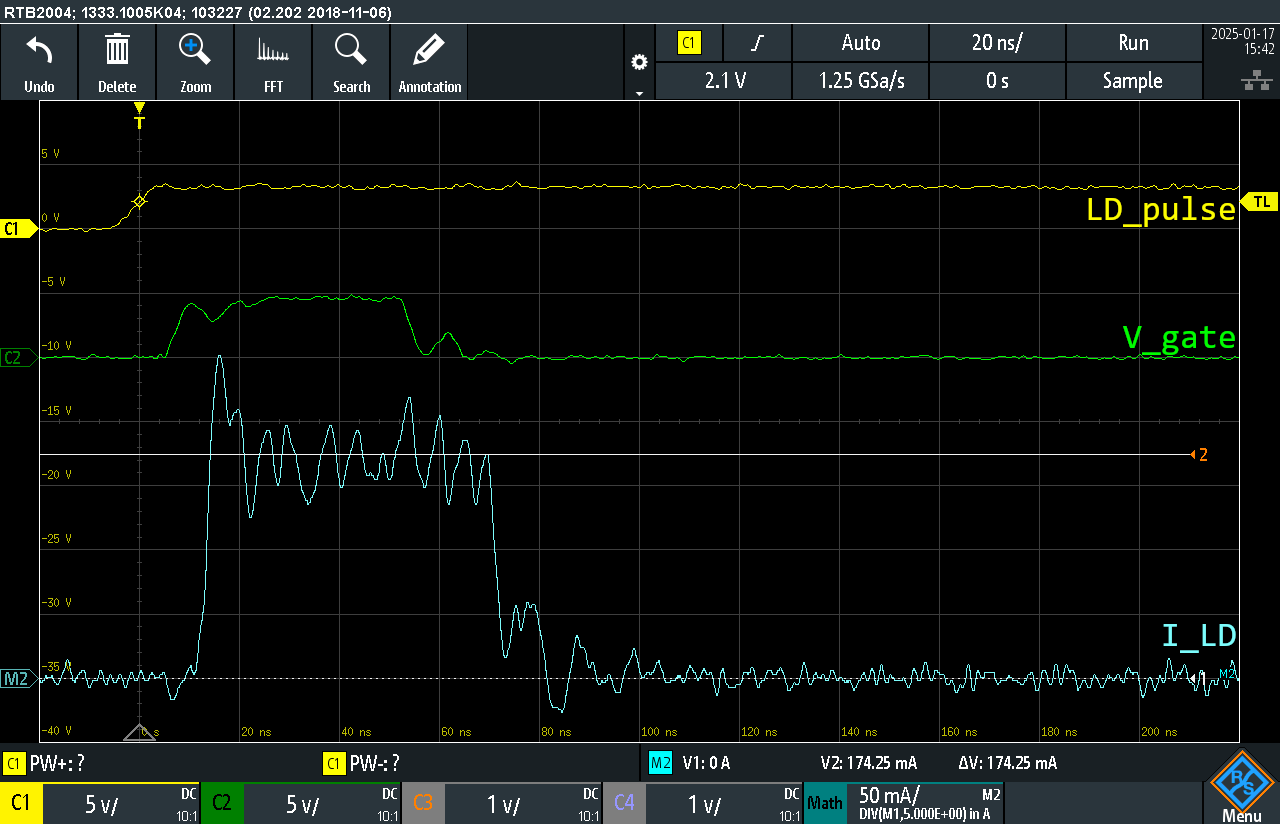
\includegraphics[width=0.7\textwidth]{../documentation/graphics/signalpfad_sender_ld_strom.png}
    \end{figure}

    \iconoptical
\end{frame}

\begin{frame}{ToF-Messungen via Spiegel}
    \begin{figure}
        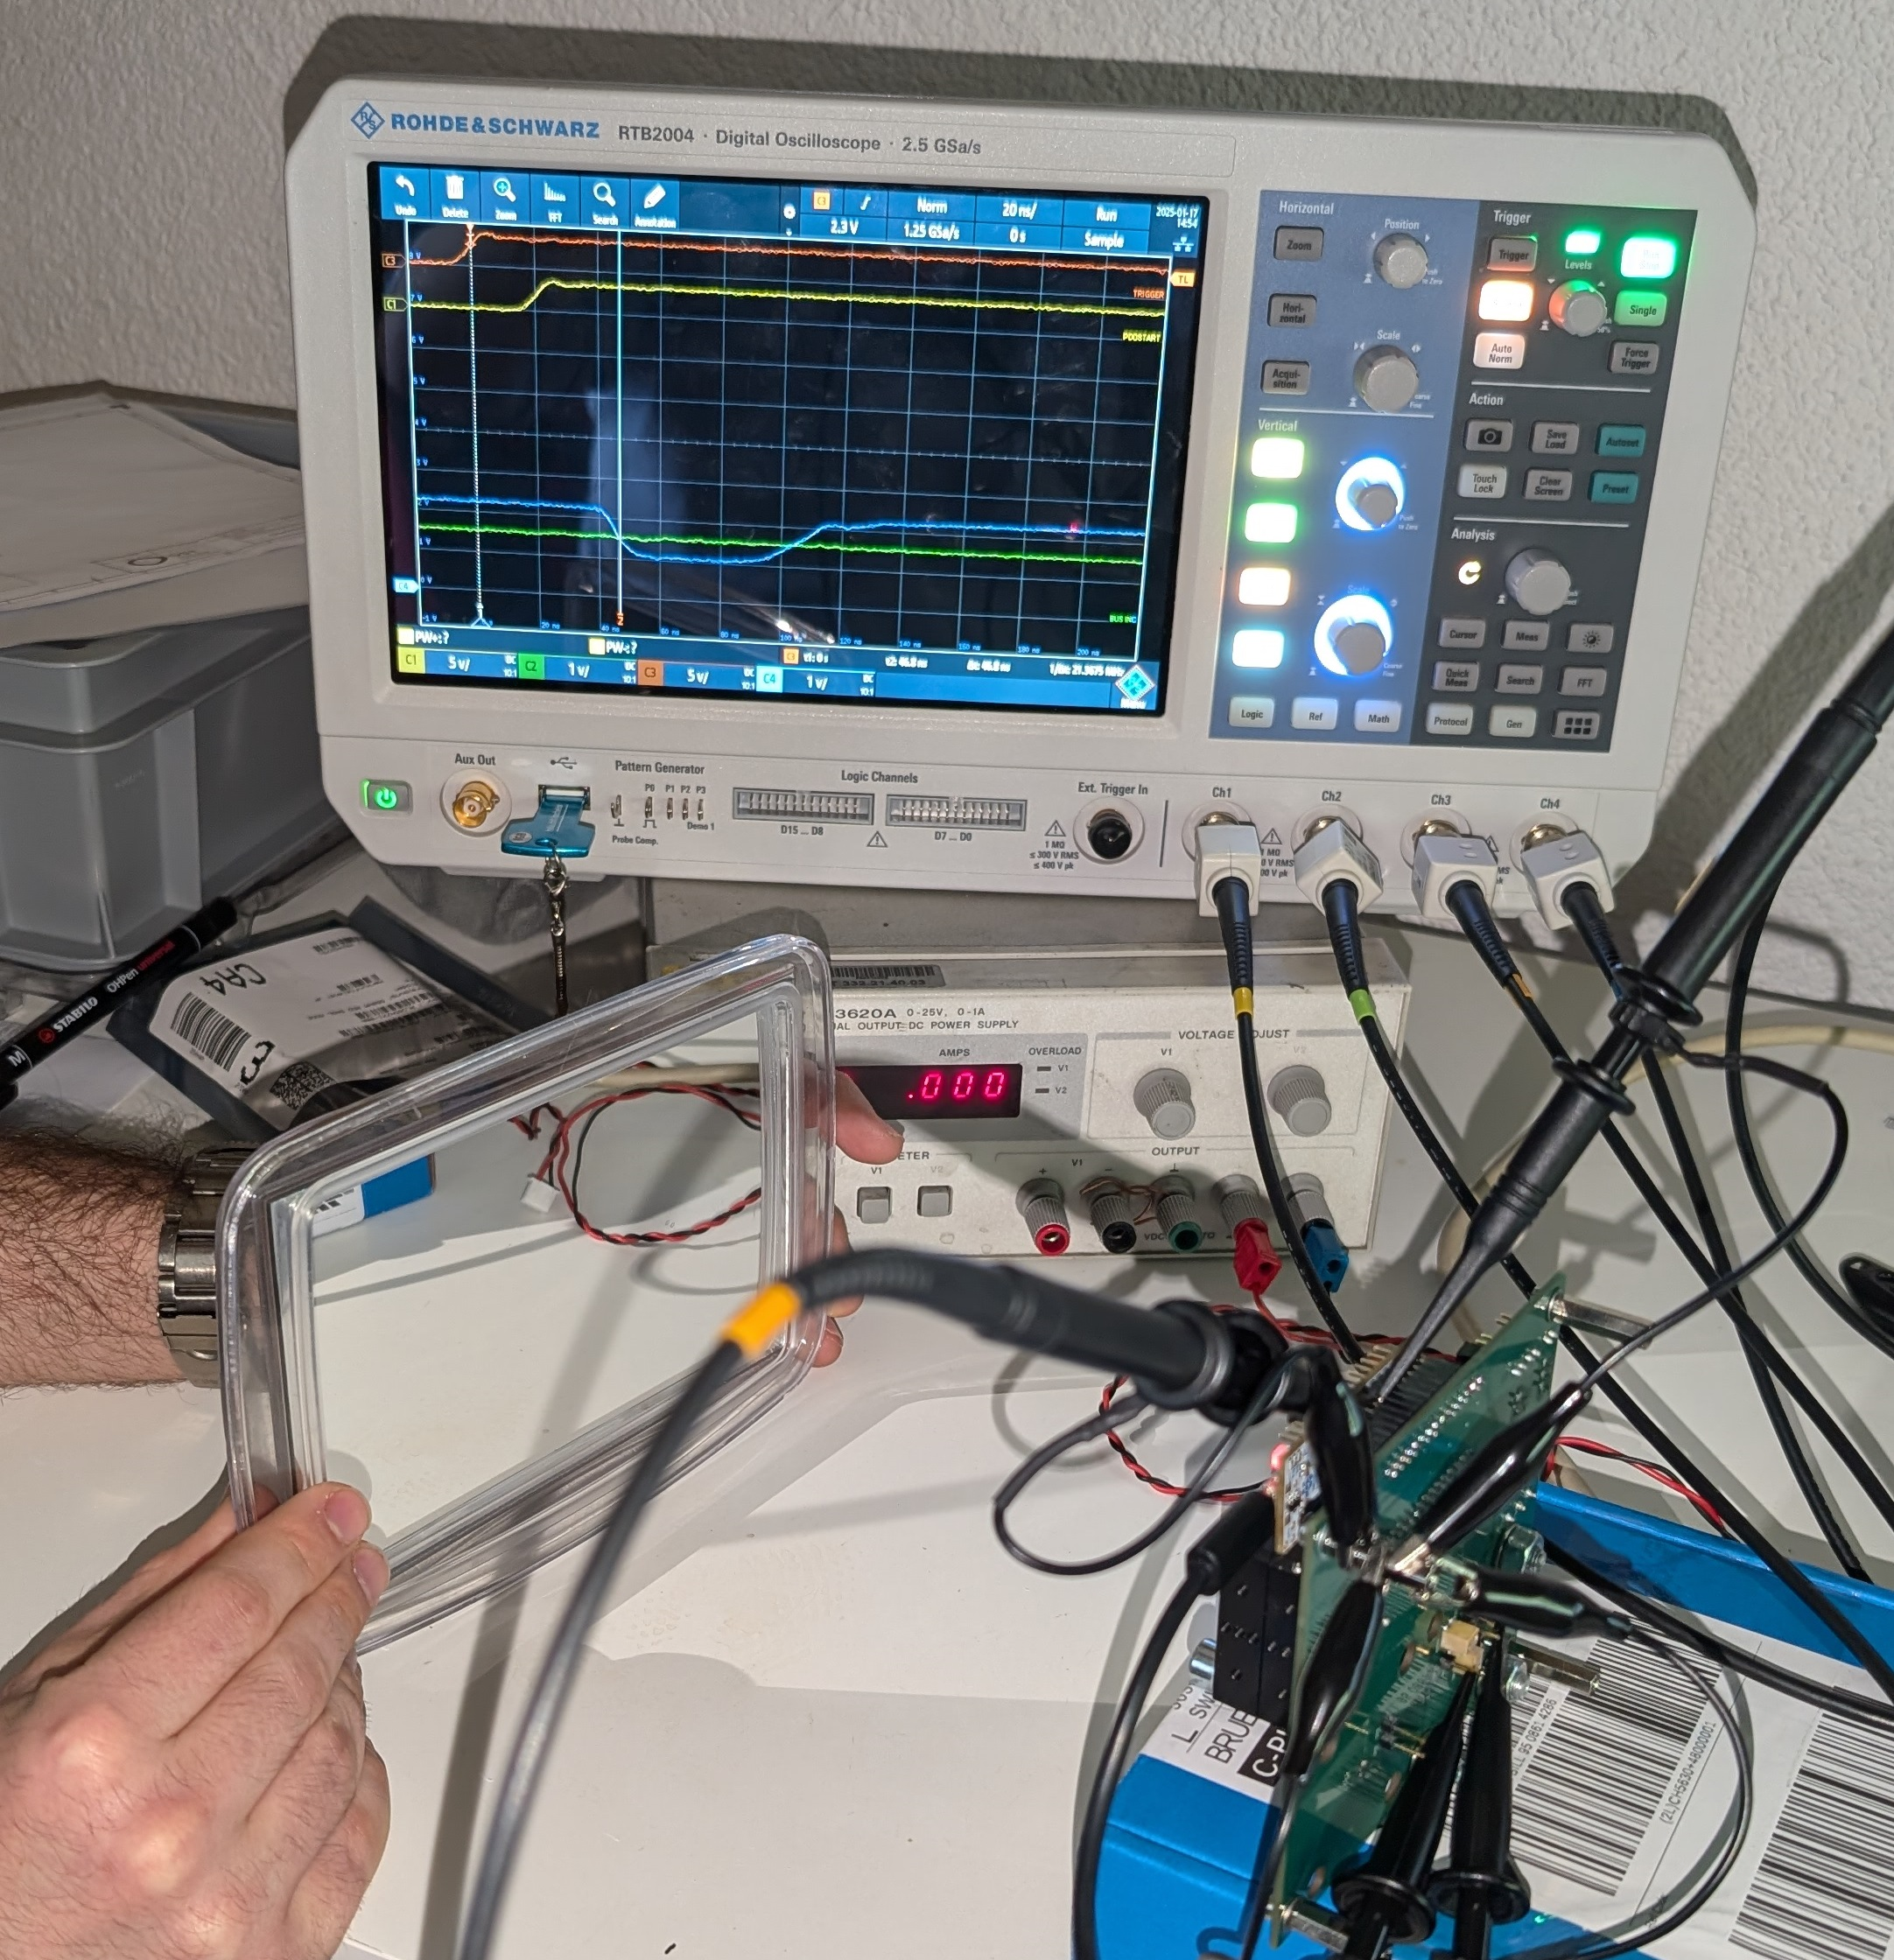
\includegraphics[width=0.45\textwidth]{../documentation/graphics/spiegel_setup.jpg}
    \end{figure}

    \iconoptical
\end{frame}

\begin{frame}{ToF-Messungen via Spiegel: DSO}
    \begin{figure}
        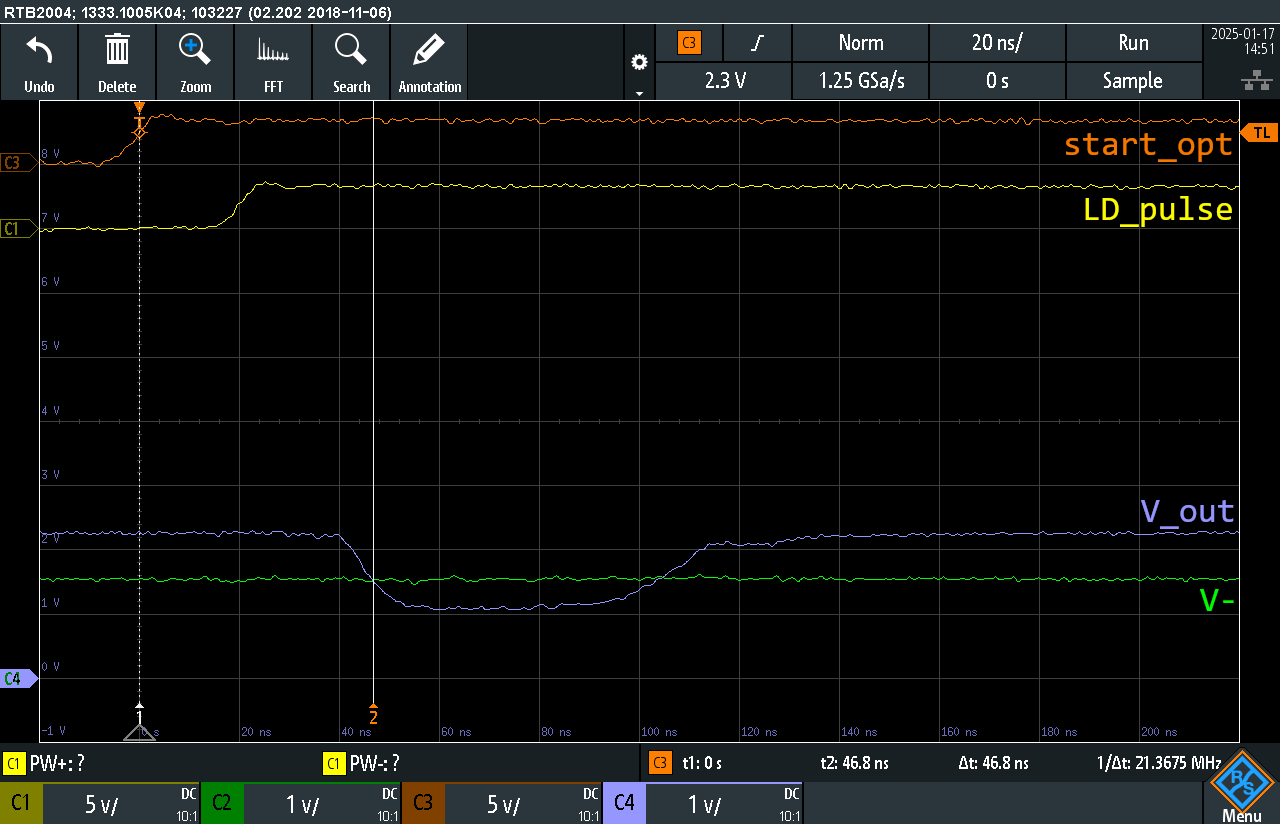
\includegraphics[width=0.7\textwidth]{../documentation/graphics/spiegel_12cm_dso_ok.png}
    \end{figure}

    \iconoptical
\end{frame}

\begin{frame}{ToF-Messungen via Spiegel: Resultate}
    \begin{figure}
        \includesvg[width=0.8\textwidth]{../documentation/graphics/spiegel_unterschiedliche_distanzen.svg}
    \end{figure}

    \iconoptical
\end{frame}

\begin{frame}{ToF-Messungen via Spiegel: Auswertung}
    \begin{table}
        \mytable
            {|l|l|l|}
            {\textbf{Distanz zum Spiegel} & \textbf{Mittelwert} & \textbf{Standardabweichung}}
            {\distance & \mean & \stddev}
            {../documentation/tables/spiegel_unterschiedliche_distanzen.csv}
    \end{table}

    \onslide<2->{
        \begin{equation*}
            \begin{split}
                \Delta ToF_{meas} &\approx 0.6~ns\\
                \Delta ToF_{calc} &= \frac{\Delta L}{c} = \frac{10~cm}{3 \cdot 10^8~m/s} = 0.33~ns
            \end{split}
        \end{equation*}
    }

    \iconoptical
\end{frame}

\begin{frame}{ToF-Messungen via Spiegel: Drift}
    \begin{figure}
        \includesvg[width=0.8\textwidth]{../documentation/graphics/spiegel_unterschiedliche_distanzen_linear.svg}
    \end{figure}

    \iconoptical
\end{frame}

\begin{frame}{ToF-Messungen via Spiegel: $>$30 cm}
    \begin{figure}
        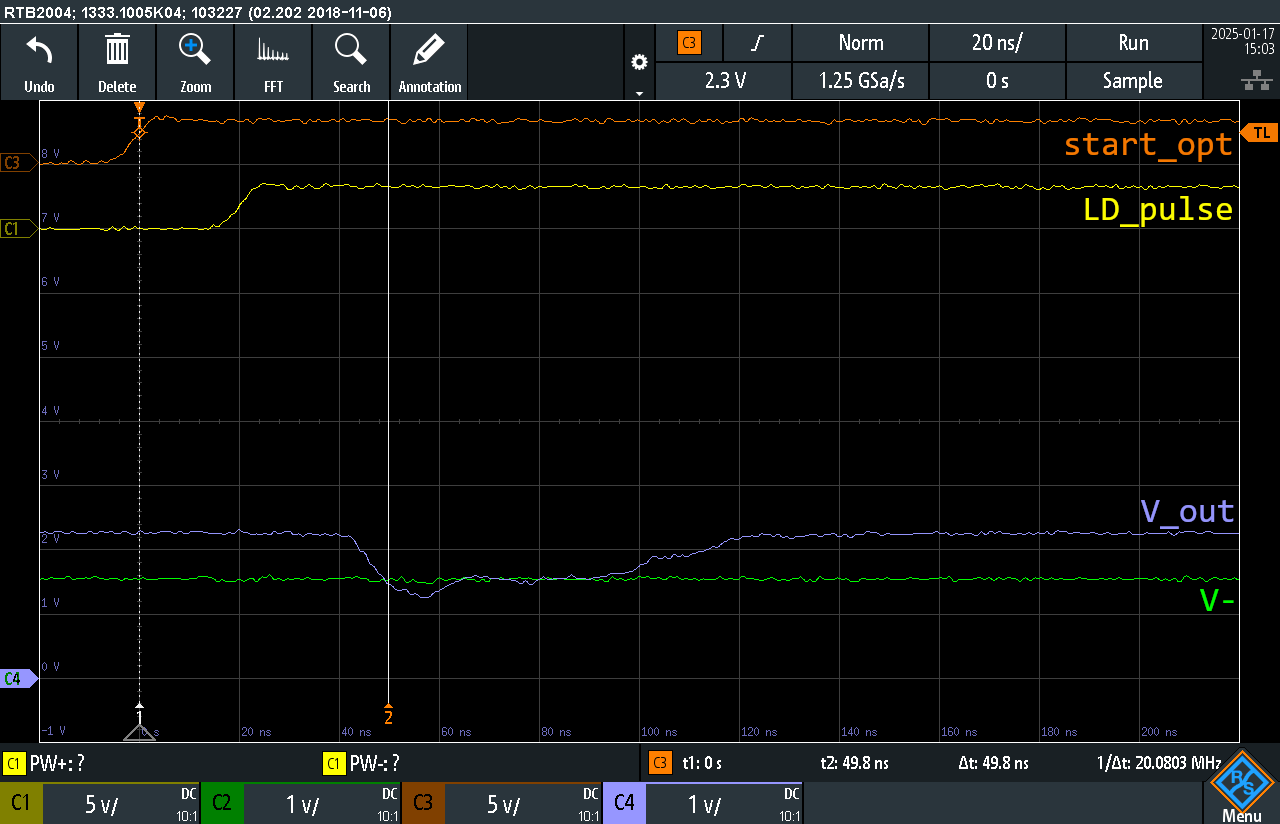
\includegraphics[width=0.7\textwidth]{../documentation/graphics/spiegel_30cm_dso_nok.png}
    \end{figure}

    \iconoptical
\end{frame}

\begin{frame}{ToF-Messungen via Wand}
    \begin{itemize}
        \item Leider Optik noch nicht dafür ausgelegt
    \end{itemize}

    \iconoptical
\end{frame}
